\documentclass[11pt,a4paper,twoside,openright]{book}

%%%% PACCHETTI PER LE IMMAGINI
\usepackage[dvips]{graphicx}
\graphicspath{ {./immagini/} }
\usepackage{float} %per posizionare le immagini nel posto corretto con "H"
\usepackage{subcaption}

%%%% PACCHETTI NON UTILIZZATI
%\usepackage{tabularx}
%\usepackage{subfigure}
%\usepackage{afterpage}
%\usepackage{amsmath,amssymb}            
%\usepackage{rotating}

%%%% ALTRI PACCHETTI
\usepackage{fancyhdr}
\usepackage{geometry}
\usepackage{hyperref}
\usepackage{multicol}

%%%% PACCHETTI PER CODICE
\usepackage[dvipsnames]{xcolor}
\usepackage[newfloat]{listings}
\renewcommand{\lstlistingname}{Codice}
\renewcommand{\lstlistlistingname}{Elenco del codice}
\definecolor{my-red}{rgb}{0.3,0,0}
\definecolor{my-grey}{rgb}{0.95,0.95,0.95}
\lstdefinestyle{my-style}{
    showstringspaces=false,
    basicstyle=\ttfamily\small,
    commentstyle=\color{my-red},
    backgroundcolor=\color{my-grey},
    language=bash,
    literate = {\$\#}{{{\$\#}}}2,
    breaklines=true
}
\lstset{style=my-style}

% per sillabazione
\hyphenation{a-gen-tiz-za-zio-ne}

%\setlength{\paperwidth}{16cm}
%\setlength{\paperheight}{24cm}
%\setlength{\oddsidemargin} {2. cm}
%\setlength{\evensidemargin} {2. cm}
%\addtolength{\oddsidemargin} {-0.4 cm}
%\addtolength{\evensidemargin} {-0.4 cm}
\geometry{
    paper=a4paper,
    margin=3cm,
    headheight=13.6cm
}

\linespread{1.1}

\usepackage[italian]{babel}
\usepackage[utf8]{inputenc}
\usepackage{csquotes} % per testo fra virgolette
\renewcommand{\captionfont}{\normalfont \sffamily \itshape \small}

\pagestyle{empty}

\begin{document}
\thispagestyle{empty}
\vspace*{-1. cm}
\begin{center}
  \Large
  \textbf{UNIVERSIT\`A DI MODENA E REGGIO EMILIA}\\
  
  \vspace{0.25 cm}
  \Large
  Dipartimento di Ingegneria Enzo Ferrari\\
  Corso di Laurea in Ingegneria Informatica\\
  \vspace*{5. cm} \LARGE

  \textbf{INSTALLAZIONE E CONFIGURAZIONE DI SHARELATEX SU MACCHINA VIRTUALE CON L'AUSILIO DELLA PIATTAFORMA DOCKER}\\
  
\end{center}

\vspace*{2.5 cm}
\Large

\begin{flushleft}
  \textbf{Relatore:}\\
  Prof. Ing. Costantino Grana\\
  \vspace*{0.25 cm}
  \textbf{Correlatore:}\\
  Dott. Ing. Federico Bolelli 
\end{flushleft}

\vspace*{0.5 cm}

\begin{flushright}
  \textbf{Candidato:}\\
  Cristian Mercadante\\
  Matricola 96980
\end{flushright}

\vspace*{3 cm}

\begin{center}
  Anno Accademico 2017-2018
\end{center} \clearpage
\normalsize



%\thispagestyle{empty} \normalfont \cleardoublepage
%\vspace*{3.5cm}

\large
\begin{flushright}
\itshape{Ai miei genitori, Paolo e Adriana,per avermi dato la possibilità\\di raggiungere questo traguardo.}
\end{flushright}


\thispagestyle{empty}  \cleardoublepage
\frontmatter
\newpage

\tableofcontents
\listoffigures


%\thispagestyle{empty} \vspace*{.75truecm} \cleardoublepage
%\chapter*{Ringraziamenti}

\addcontentsline{toc}{chapter}{Ringraziamenti}

Ringrazio tutti coloro che mi hanno supportato e aiutato in questi tre anni, a partire dall'Ing. Federico Bolelli, che è sempre stato disponibile durante lo svoglimento del progetto. Ringrazio i miei colleghi, con cui ho condiviso bei momenti e che mi hanno sostentuto. Ringrazio gli amici del mio paese, che conosco da quando ero bambino, che mi hanno sempre incoraggiato e fatto forza. Ringrazio la mia famiglia, in particolare i miei genitori, Adriana e Paolo, che mi hanno dato la possibilità di raggiungere questo traguardo.


\thispagestyle{empty} \vspace*{.75truecm} \normalfont \cleardoublepage
\pagestyle{fancy} \renewcommand{\chaptermark}[1]{\markboth{\chaptername\ \thechapter.\ #1}{}}
\renewcommand{\sectionmark}[1]{\markright{\thesection.\ #1}}         
\fancyhead[LE,RO]{\bfseries \thepage}
\fancyhead[RE]{\bfseries\leftmark}
\fancyhead[LO]{\bfseries\rightmark}     
\renewcommand{\headrulewidth}{0.3pt}

\mainmatter

\chapter{Introduzione}
\label{Introduzione}
\thispagestyle{empty}

Il seguente elaborato descrive le fasi di installazione e configurazione del software \emph{ShareLaTeX} su una macchina virtuale ospitata da un server all'interno del Dipartimento di Ingegneria Enzo Ferrari dell'Università di Modena e Reggio Emilia.

\section{Motivazioni}
L'applicazione ShareLaTeX è assai utilizzata all'interno del gruppo di ricerca del dipartimento. Professori, dottori e dottorandi utilizzano quest'applicazione per scrivere, memorizzare e aggiornare le proprie pubblicazioni scientifiche ed ingegneristiche scritte in \LaTeX. Il gruppo di ricerca AImageLab necessita di un'installazione di ShareLaTeX su un server locale, per far fronte a due esigenze:
\begin{itemize}
    \item Evitare problemi di disconnessione che possano compromettere lo stato e la modifica dei documenti. Mediante connessione in rete locale al servizio vengono scongiurati problemi di questo tipo.
    \item Conservare progetti e documenti sul server dell'ateneo in modo sicuro.
\end{itemize}
Pertanto si è pensato di sfruttare le guide e i tool messi a disposizione dagli sviluppatori dell'applicazione per installare un'instanza locale di ShareLaTeX all'interno dell'ateneo. Si è poi deciso, per permettere agli utenti di utilizzare il servizio anche al di fuori della rete universitaria, di rendere accessibile il sito anche all'esterno dell'ateneo all'indirizzo \url{sharelatex.ing.unimore.it}.

\section{Obiettivi}
L'obiettivo di questo progetto è l'installazione di ShareLaTeX e la sua configurazione per il Dipartimento di Ingegneria Enzo Ferrari. Inoltre si vuole che il sistema sia facilmente manutenibile in fase di aggiornamento dei suoi componenti.

\section{Strumenti}
Al fine dell'installazione, gli sviluppatori di ShareLaTeX hanno fornito un'immagine funzionante e aggiornata del sistema sulla piattaforma Docker. È disponibile la guida ufficiale d'installazione all'indirizzo \url{github.com/sharelatex/sharelatex/wiki}. Questa presenta sia una \enquote*{Quick Start Guide}, sia paragrafi dettagliati sulle varie fasi d'installazione.

\section{Contenuti}
Si presenta ora un riassunto di ciò che sarà affrontato nei capitoli successivi. I capitoli 2 e 3 affronteranno aspetti tecnici e teorici, mentre i capitoli 4, 5 e 6 affronteranno aspetti pratici, legati all'installazione di ShareLaTeX.
\begin{itemize}
    \item Nel capitolo 2 si parlerà di ShareLaTeX, delle sue funzionalità e delle sue potenzialità.
    \item Nel capitolo 3 si parlerà della piattaforma Docker, dei suoi componenti, del suo funzionamento e delle sue potenzialità.
    \item Nel capitolo 4 si spiegherà come installare Docker e il tool Docker Compose.
    \item Nel capitolo 5 si spiegherà come personalizzare e configurare ShareLaTeX.
    \item Nel capitolo 6 si spiegherà come eseguire backup, ripristino e aggiornamento del sistema.
\end{itemize}
\chapter{ShareLaTeX}
\label{ShareLaTeX}
\thispagestyle{empty}

ShareLaTeX è uno strumento assai diffuso all'interno della comunità scientifica e accademica. È un editor di documenti in linguaggio \LaTeX ~che presenta numerose funzionalità che lo distinguono dai normali editor.

\section{Funzionalità}

ShareLaTeX è un'applicazione web che consente agli utenti di creare, importare, modificare e gestire progetti \LaTeX. La caratteristica che contraddistingue ShareLaTeX è l'essere un editor collaborativo. Nel momento in cui l'autore di un documento non è un singolo utente, ma un gruppo, risulta difficile sincronizzare le modifiche apportate al progetto e lo stato dei file con un normale editor \LaTeX. ShareLaTeX consente la condivisione dei documenti con più utenti, ai quali possono essere concessi sia privilegi di lettura che di scrittura. Qualunque modifica apportata al progetto sarà visibile in tempo reale a tutti i collaboratori connessi in quel momento e i file rimarranno consistenti. I progetti conservano inoltre lo storico delle modifiche, quindi è possibile ripristinare ciascun file alla versione precedente, oppure ripristinare un file eliminato.

\section{Interfaccia}
ShareLaTeX offre un'interfaccia utente semplice e immediata. Ogni utente iscritto possiede la sua homepage con i progetti creati, dalla quale può decidere se aprire un progetto esistente o crearne uno nuovo.
\begin{figure}[h]
    \centering
    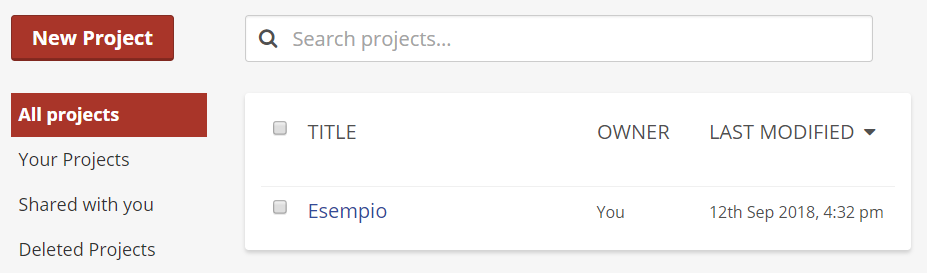
\includegraphics[width=\textwidth]{immagini/homepage.PNG}
    \caption{Homepage di ShareLaTeX}
    \label{fig:sharelatex_homepage}
\end{figure}

L'interfaccia dell'editor è divisa in tre parti:
\begin{itemize}
    \item Una colonna di navigazione fra i file del progetto, dalla quale si possono non solo creare nuovi file e cartelle, ma anche importarli da locale o dal web.
    \item La finestra di editor vera e propria, dove l'utente scrive testo e comandi \LaTeX, con evidenziazione della sintassi e autocompletamento dei comandi.
    \item La finestra di anteprima del documento, che presenta l'esito della compilazione.
\end{itemize}
\begin{figure}[h]
    \centering
    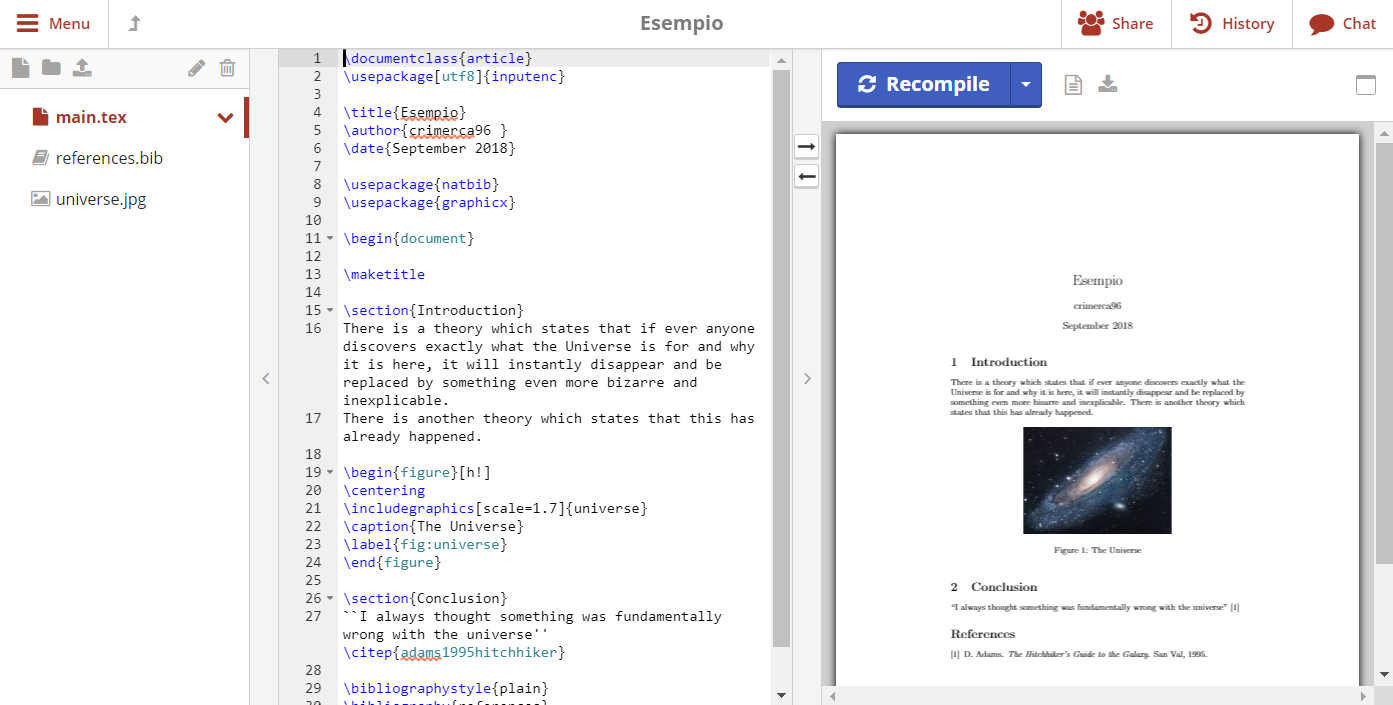
\includegraphics[width=\textwidth]{immagini/editor.PNG}
    \caption{Interfaccia dell'editor di ShareLaTeX}
    \label{fig:sharelatex_editor}
\end{figure}
Nell'editor è inoltre possibile condividere il progetto con altri utenti, visualizzare la cronologia delle modifiche e la chat di progetto, mediante i tre pulsanti in alto a destra.
Il pulsante \enquote*{Menu} in alto a sinistra mostra una colonna aggiuntiva dalla quale è possibile:
\begin{itemize}
    \item Scaricare il codice sorgente del progetto e il PDF di output.
    \item Contare le parole.
    \item Selezionare uno fra i compilatori disponibili: pdfLaTeX, \LaTeX, XeLaTeX e LuaLaTeX.
    \item Selezionare il documento principale da cui iniziale la compilazione.
    \item Indicare il linguaggio di scrittura per la correzione dello spelling.
    \item Attivare o disattivare l'auto-completamento del testo, l'auto-chiusura delle parentesi e il controllo del codice.
    \item Selezionare il tema della schermata dell'editor e la dimensione del font.
    \item Mostrare/modificare le scorciatoie da tastiera dell'editor.
\end{itemize}

\section{Database}
ShareLaTeX necessita di due DBMS per funzionare: MongoDB e Redis. In seguito si presentano tali servizi, mettendo in luce i loro punti di forza.

\subsection{MongoDB}
MongoDB \cite{mongodb} è un DBMS non relazionale, anche detto NoSQL. È un progetto open source con licenza GNU AGPL v3.0. Anziché essere basato su tabelle e dipendenze fra queste, MongoDB utilizza il modello a documenti. Questi consentono di strutturare i dati in maniera efficiente da processare per le macchine, ma allo stesso tempo naturale e facile per l'essere umano da leggere. DBMS relazionali, specialmente se di grandi dimensioni, possono risultare difficili da comprendere, da aggiornare, inefficienti e spesso gli sviluppatori devono modellare le proprie applicazioni sulle esigenze del DBMS. MongoDB invece si adatta alle esigenze di chi sviluppa, concedendo loro di memorizzare dati in maniera più libera, senza la preoccupazione che un piccolo cambiamento possa compromettere lo stato della base di dati. Inoltre MongoDB può nativamente coordinare molteplici server per immagazzinare dati. È quindi definito \enquote*{distributed database}. È tollerante ai guasti, qualora siano stati previsti server secondari ridondanti. È scalabile, poichè può immagazzinare dati in più server per bilanciare il carico. Infine è possibile migrare facilmente i database, in modo da conservare i dati vicino agli utenti per garantire accessi veloci.

ShareLaTeX utilizza MongoDB come database principale.

\subsection{Redis}
Redis \cite{redis} è un DBMS non relazionale, anche detto NoSQL. È un progetto open source con licenza BSD 3-Clause. Redis è un archivio di strutture dati, utilizzato sia come database che come meccanismo di caching. Infatti il punto di forza di Redis è la velocità, perché funziona completamente in memoria RAM ed è scritto in C. Utilizza strutture dati predefinite per migliorare le performance: list, sets, sorted sets, hashes, hyperloglogs, bitmaps, geospatial indexes, bitfields, streams e strings. Redis, oltre ad essere completamente \enquote*{in-memory}, permette la persistenza dei dati e un'alta disponibilità grazie a repliche e backup.

ShareLaTeX utilizza Redis principalmente come meccanismo di caching.


\section{Sviluppo e distribuzione}
ShareLaTeX è un'azienda fondata da Henry Oswald e James Allen. Il software ha licenza GNU AGPL v3.0 e il codice sorgente è liberamente accessibile su GitHub \cite{sharelatex_gh}. Nel corso degli anni la community ha contribuito alla crescita e al miglioramento della piattaforma. La versione online di ShareLaTeX propone diversi piani di abbonamento all'utente, flessibili su base mensile e annuale, con prezzo dimezzato per gli studenti. I vari abbonamenti differiscono per il numero di collaboratori per progetto e per la presenza delle funzionalità aggiuntive di sincronizzazione con Dropbox e GitHub.

Gli sviluppatori hanno fornito una guida per l'installazione e configurazione dei ShareLaTeX \cite{sharelatex_wiki}. Tale guida è stata usata come riferimento principale per lo svolgimento di questo progetto. Gli sviluppatori hanno inoltre fornito un'immagine aggiornata e funzionante del sistema per la piattaforma Docker \cite{sharelatex_docker_hub}.

\section{Overleaf v2}
Il 20 luglio 2017 ShareLaTeX annuncia la fusione con Overleaf, un altro software per l'editing collaborativo di progetti \LaTeX. Dall'unione nasce Overleaf v2 \cite{overleaf_v2}. Dal 4 settembre 2018 ShareLaTeX non è più disponibile e tutti gli account creati sono stati esportati sulla nuova piattaforma. Il team ha comunque dichiarato che ShareLaTeX continuerà a crescere e ad essere open source.

L'interfaccia della homepage e dell'editor sono le medesime di ShareLaTeX, con qualche cambiamento estetico. Inoltre, è possibile scrivere utilizzando la nuova funzionalità chiamata \enquote*{Rich text}, che consente di visualizzare nella finestra di scrittura un'interfaccia più user-friendly, adatta a chi non è esperto di \LaTeX ~e dei suoi comandi.
\begin{figure}[h]
    \centering
    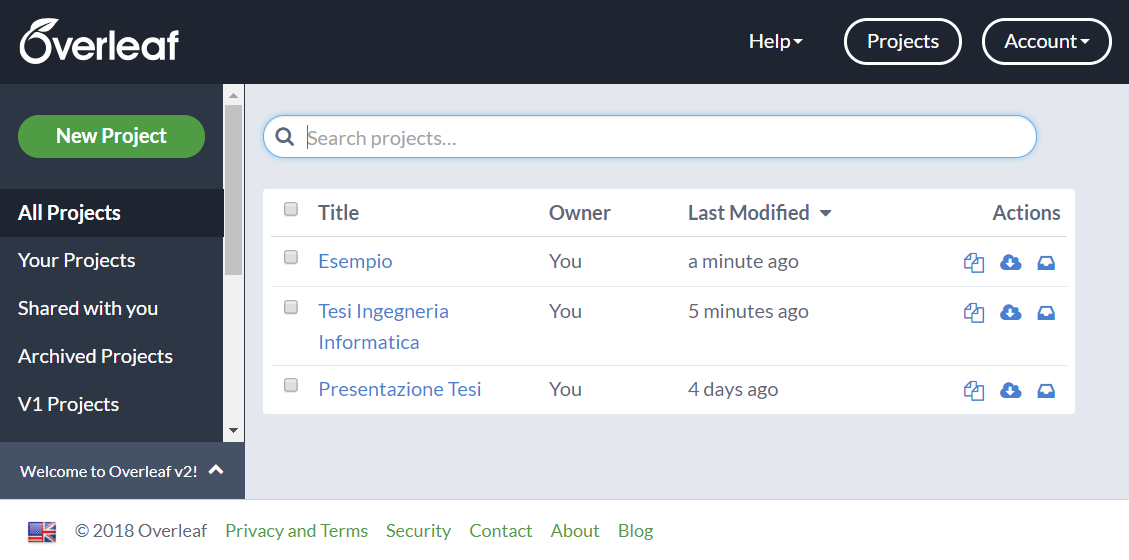
\includegraphics[width=\textwidth]{immagini/overleaf_homepage.PNG}
    \caption{Homepage di Overleaf v2}
    \label{fig:overleaf_homepage}
\end{figure}
\begin{figure}[h]
    \centering
    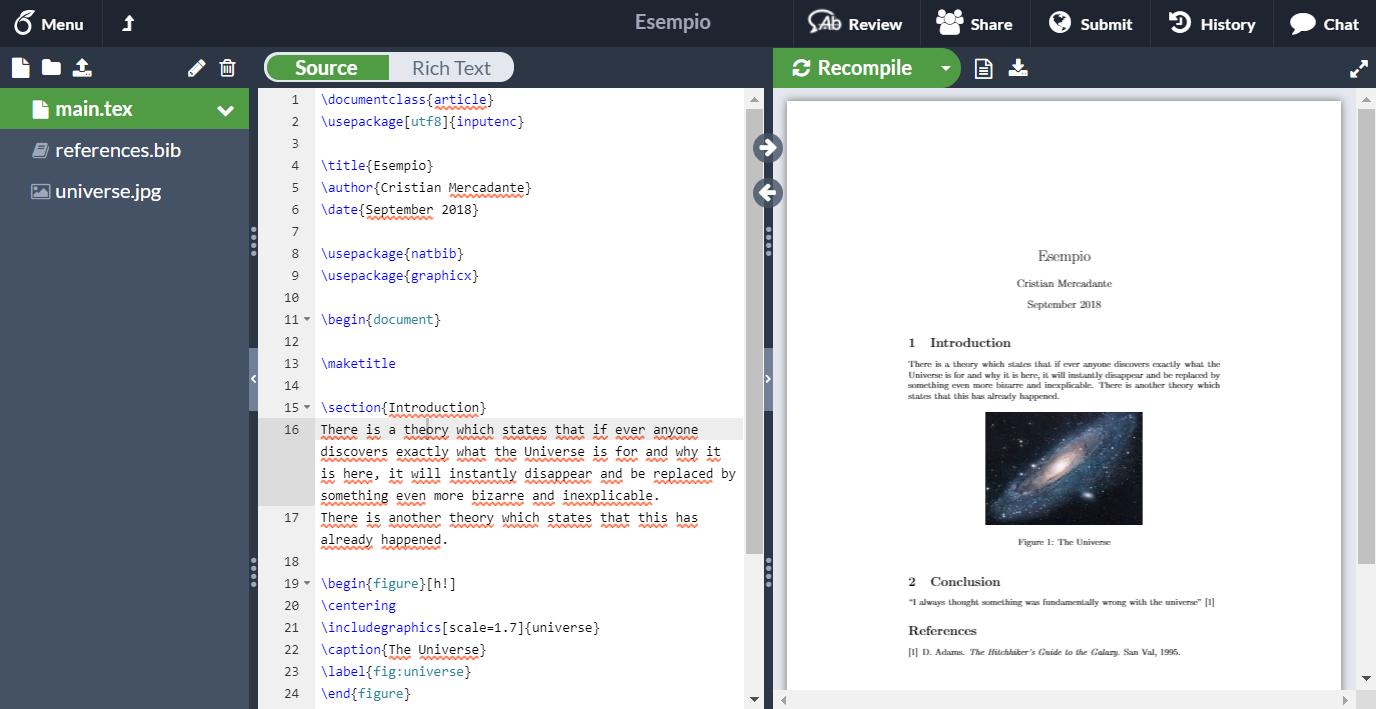
\includegraphics[width=\textwidth]{immagini/overleaf_editor.PNG}
    \caption{Interfaccia dell'editor di Overleaf v2}
    \label{fig:overleaf_editor}
\end{figure}


\chapter{Docker}
\label{Docker}
\thispagestyle{empty}

Docker è una piattaforma per sviluppare, spedire e avviare applicazioni usando la tecnologia dei container. Il progresso dell'industria tecnologica procede ad un ritmo elevatissimo e sempre più aziende hanno bisogno di strumenti affidabili e facilmente scalabili a seconda delle esigenze. La piattaforma Docker è lo strumento all'avanguardia che permette la consegna ed installazione di servizi in semplicità e sicurezza, mediante componenti leggeri e standard, assai portabili e aggiornabili, chiamati container. Questi non solo sono utilizzati per sviluppare nuovi servizi e micro-servizi, ma anche per eseguire applicazioni esistenti, preparandole ad una futura modernizzazione. Infatti i vantaggi della piattaforma hanno convinto l'industria, che oggi confida sempre più su questa tecnologia, costruendo piattaforme di container.

\section{Versioni}
Docker è un software disponibile per diversi sistemi operativi fra cui sistemi Linux (Ubuntu, Fedora, Debian, CentOS), Windows, Mac, ma anche in cloud (Amazon Web Services, Microsoft Azure). È disponibile in due versioni:
\begin{itemize}
    \item Community Edition (CE): gratuita, ideale per sviluppatori singoli e per piccoli team. Possiede le funzionalità di base della piattaforma.
    \item Enterprise Edition (EE): studiata per sviluppo aziendale e per team che sviluppano, spediscono ed eseguono applicazioni essenziali per l'impresa.
\end{itemize}

\section{Architettura, componenti e funzionamento}
Docker utilizza funzionalità di virtualizzazione del kernel Linux per avviare servizi e applicazioni in un ambiente isolato, protetto e sicuro. In seguito si descriveranno i componenti base di Docker e di come interagiscano fra loro.

\subsection{Immagini}
Un'immagine è un template con istruzioni per la creazione di container. Le immagini descrivono anche i componenti e i programmi all'interno del container e possono includere anche altre immagini. Ad esempio, è possibile indicare che sull'immagine "Ubuntu" sia installato il web server Apache ed altre applicazioni con le relative impostazioni. È possibile creare le proprie immagini, ma anche utilizzarne altre disponibili su \hyperref[docker-hub]{Docker Hub}. Per creare un immagine è necessario creare un \emph{Dockerfile} che indichi gli step per la creazione e l'avvio dell'immagine. Ogni step costituisce un layer dell'immagine: la ricreazione dell'immagine a fronte di modifiche comporterà la sola sostituzione dei layer modificati. L'operazione risulta quindi assai conveniente, leggera e veloce.

\subsection{Container}
Un container è un'istanza eseguibile di un'immagine. Ogni container possiede i propri processi, la propria memoria, i propri dispositivi e stack di rete. I container isolano quindi il proprio ambiente da quello esterno, assicurandosi che i propri applicativi funzionino sempre e in modo sicuro, indipendentemente dalle specifiche dell'host. È possibile connettere un container alla rete oppure ad altri container, assegnargli spazio di archiviazione e utilizzare lo stato attuale per creare nuove immagini. Pertanto un container è definito dalla sua immagine e dalla sua configurazione di avvio. Al riavvio di un container, ogni modifica apportata al suo stato o ai suoi dati verrà persa. È possibile introdurre la persistenza dei dati utilizzando la tecnologia dei \emph{volumi}. Questi sono completamente gestiti da Docker, sono facili da eseguire o migrare e sono utilizzabili in sicurezza da più container. La creazione di un volume consiste nella copia di una directory dal filesystem del container verso il filesystem dell'host. Docker gestisce direttamente il contenuto di queste directory. Ad esempio, a seguito del riavvio di un container, Docker carica i dati salvati sull'host all'interno della directory specificata, ripristinando il suo stato prima dello spegnimento.

\subsection{Docker Engine}
Docker Engine è un'applicazione con architettura di tipo client-server. È costituita da tre componenti:
\begin{itemize}
    \item Un processo daemon (\verb|dockerd|) che rappresenta il server.
    \item Una REST API che definisce in che modo i programmi possono interagire con il processo daemon.
    \item Un'interfaccia a linea di comando (\verb|docker|) che rappresenta il client.
\end{itemize}
Il daemon riceve richieste dal client per costruire, eseguire e distribuire container e può comunicare con altri daemon per gestire servizi Docker più complessi. Il client invece, eseguendo comandi come \verb|docker run|, utilizza le REST API, socket UNIX o interfacce di rete per comunicare col daemon. Client e server possono essere eseguiti sullo stesso host oppure su macchine differenti. Nell'\hyperref[fig:docker_engine_b]{esempio} sottostante possiamo osservare come il daemon gestisca richieste differenti. Ad esempio \verb|docker pull| ordina al server di collegarsi a \hyperref[docker-hub]{Docker Hub} per scaricare l'immagine di Redis, mentre \verb|docker run| richiede che l'immagine di Ubuntu, già disponibile localmente, sia avviata.
\begin{figure}[h]
    \begin{subfigure}{0.4\textwidth}
        \centering
        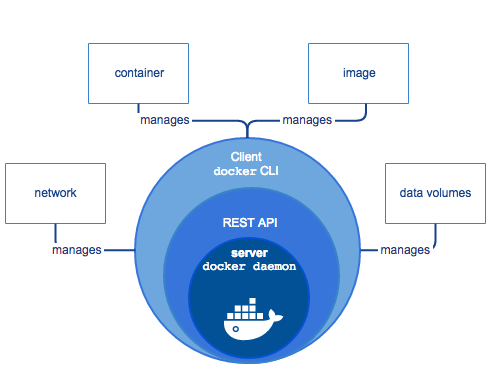
\includegraphics[width=\textwidth]{immagini/engine-components-flow.png}
        \caption{Struttura del Docker Engine}
        \label{fig:docker_engine_a}
    \end{subfigure}
    \begin{subfigure}{0.6\textwidth}
        \centering
        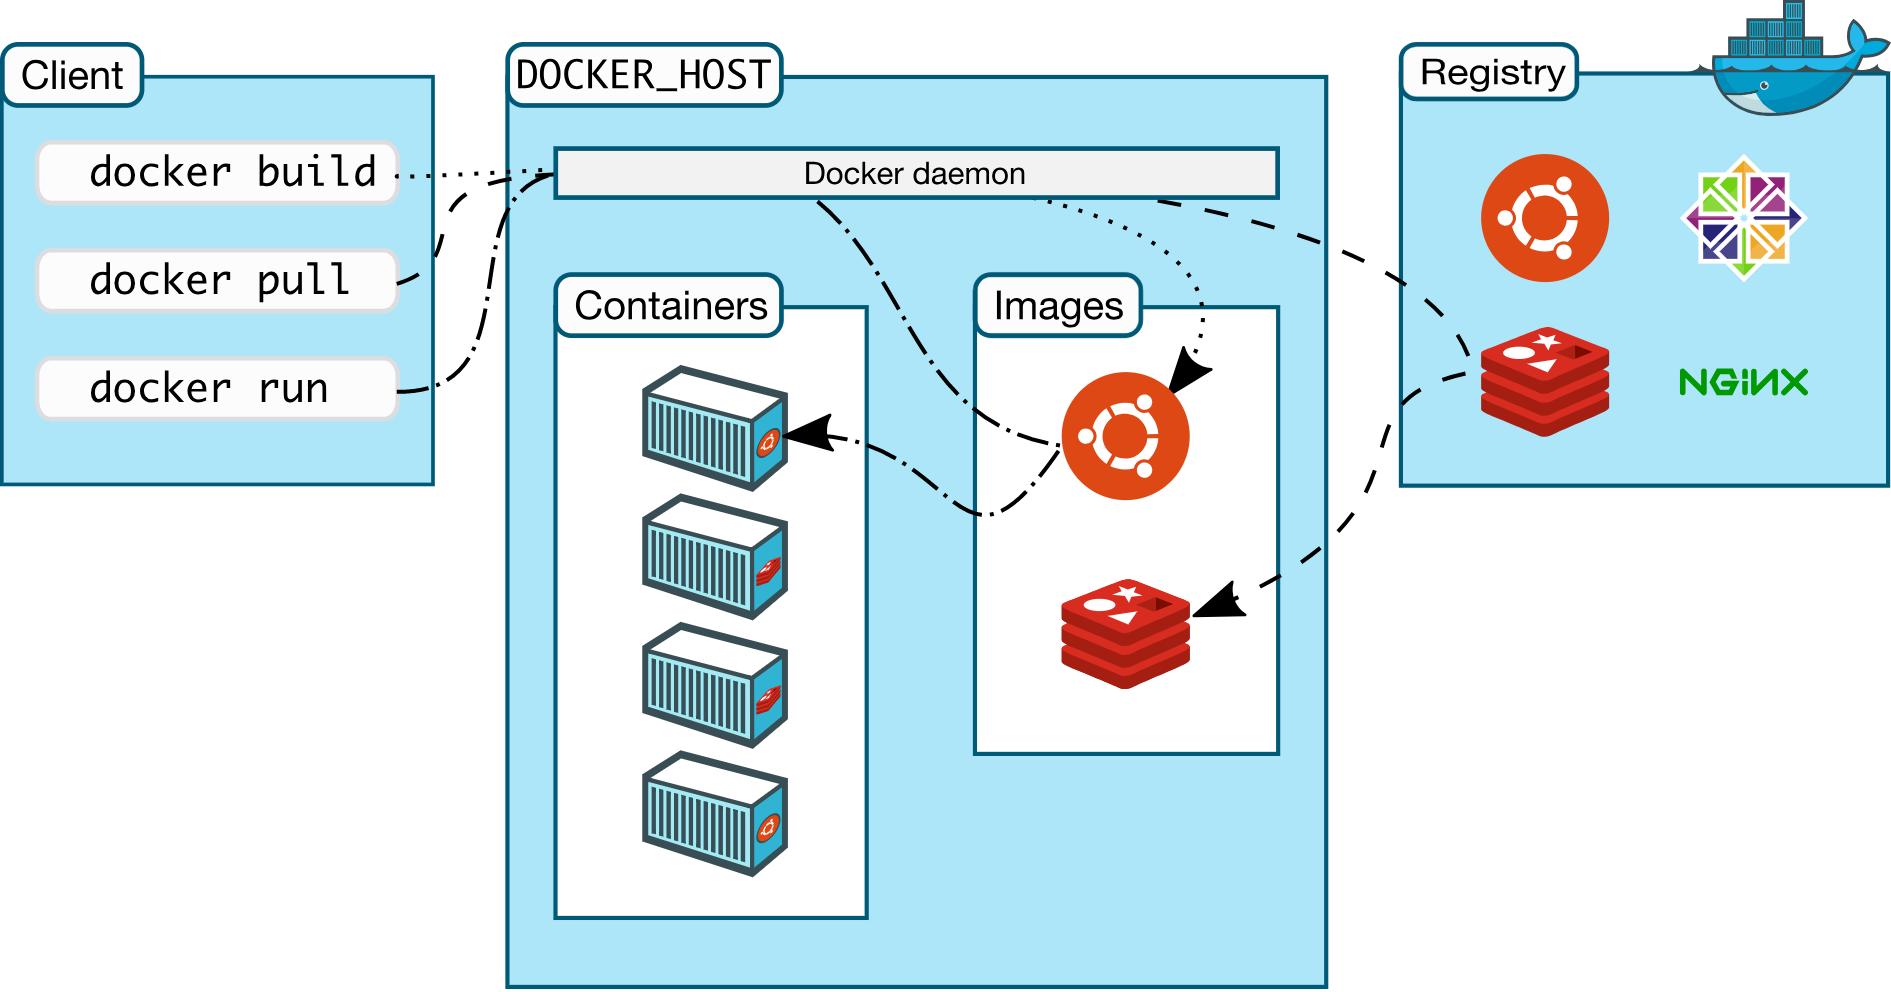
\includegraphics[width=\textwidth]{immagini/architecture.png}
        \caption{Esempio funzionamento Docker Engine}
        \label{fig:docker_engine_b}
    \end{subfigure}
    \caption{Docker Engine}
    \label{fig:docker_engine}
\end{figure}

\subsection{Docker Hub}\label{docker-hub}
Docker Hub è un servizio che consente di collegarsi a repository di immagini. Permette agli utenti di caricare e scaricare liberamente immagini di container da avviare sui propri host. Costituisce inoltre il nodo centrale per lo sviluppo, la distribuzione e gestione delle modifiche dei container. Docker Hub contiene un gran numero di repository ufficiali, pubblici e certificati dai fornitori. Fra questi si citano NGINX, Redis, MongoDB, Ubuntu, PostgreSQL, Node.js, MySQL, Tomcat e molti altri.

\subsection{Docker Compose}
Docker Compose è uno strumento per definire ed avviare servizi multi-container mediante un file YAML chiamato \verb|docker-compose.yml|. In questo file sono contenute tutte le informazioni per la configurazione dei vari servizi. È possibile infatti modificare diversi campi per cambiare il comportamento del container, ad esempio indicando l'immagine o il Dockerfile di riferimento, creando dipendenze da altri servizi, associandogli un numero di porta, indicando comandi da eseguire all'avvio e molto altro. Con lo stesso file si possono gestire più container, le loro dipendenze e avviarli in contemporanea. Pertanto Docker Compose risulta uno strumento utile sia in fase di sviluppo, dove può essere utilizzato per creare ambienti controllati con cui interagire facilmente e testare la propria applicazione, che in fase di distribuzione, quando non è più richiesto all'installatore di preparare l'ambiente per l'applicazione, ma solo di eseguire il comando \verb|docker-compose up|.

Segue un estratto di \verb|docker-compose.yml| utilizzato per il progetto:
\lstinputlisting[lastline=17, caption={Esempio di docker-compose.yml}, captionpos=b]{script/docker-compose.yml}
È indicata la versione del formato del file, seguita dai servizi da gestire. Per ShareLaTeX si impone con \verb|restart: always| che in caso di errore nel container, questo si riavvierà sempre. A seguire si specifica il nome dell'immagine di riferimento, il nome del container che verrà creato, le dipendenze, la priorità del container sugli altri, il numero di porta, i collegamenti con altri container e infine i volumi da montare sull'host per la persistenza dei dati.
 
\section{Tecnologia sottostante}
Docker è scritto in linguaggio GO ed utilizza diverse funzionalità del kernel Linux per eseguire container in ambienti controllati, in modo leggero e veloce. Tali funzionalità sono raccolte all'interno della libreria \emph{libcontainer}, che permette a Docker Engine di gestire il ciclo di vita dei container.

\subsection{Namespaces}
Docker Engine utilizza la tecnologia dei namespaces per creare un gruppo di namespaces all'avvio di ogni container. In tal modo ad ogni container è associato un ambiente isolato, ottenuto come risultato di una partizione delle risorse del kernel host. Pertanto i namespaces limitano ciò che un container vede e quindi più utilizzare. I namespaces utilizzati in Docker sono:
\begin{itemize}
    \item PID: per isolare i processi appartenenti ad un determinato container da quelli in esecuzione sull'host o in altri container.
    \item NET: per la gestione delle interfacce di rete.
    \item IPC: per la gestire gli accessi alle risorse di Inter Process Communication.
    \item MNT: per gestire i punti di mount del filesystem.
    \item UTS: per dare a ogni container un hostname.
\end{itemize}
%È importante sottolineare che ogni processo è in un namespace di ogni tipo. Ad esempio, processi con un un certo PID namespace possono vedere solo processi nello stesso PID namespace.

\subsection{Cgroups}
Docker Engine utilizza un'altra tecnologia chiamata cgroups, ovvero control groups, per limitare la quantità di risorse utilizzate da un container. Infatti le risorse hardware dell'host sono limitate e devono essere ripartite e condivise fra i container, impostando limiti e vincoli di utilizzo. Cgroups dà la possibilità di limitare le risorse (si pensi alla memoria), definire priorità, misurare le risorse utilizzate e controllare processi qualora superino i limiti imposti, congelandoli e riavviandoli quando possibile.

\subsection{Union filesystems}
Union filesystem, anche detto UnionFS, è una tecnologia che consente la sovrapposizione di filesystem separati, ovvero l'aggregazione di file e directory differenti e separate per formare un singolo filesystem. Docker Engine utilizza questa tecnologia per costruire container senza duplicare file o directory. Inoltre UnionFS permette la scrittura anche su file che appaiono read-only mediante il meccanismo copy-on-write. Si ipotizzi di voler avviare più container con la stessa immagine: in memoria sarebbero presenti tante copie dei filesystem quanti sono i container avviati. Con il meccanismo copy-on-write, il filesystem utilizzato è uno, mentre tutte le modifiche apportate da ogni container risultano salvate su layer copy-on-write di dimensioni contenute. Questo spiega anche come sia possibile, una volta scritto sul filesystem di un container, avviare un secondo container dalla stessa immagine senza conservare le modifiche apportate al primo.

\subsection{Funzionamento su Windows e MacOS}
Le tecnologie precedentemente elencate sono proprie del kernel Linux. Le versioni di Docker per Windows e MacOS necessitano di un livello aggiuntivo per avviare container. In Windows è avviata una macchina virtuale Linux leggera tramite Hyper-V, mentre MacOS utilizza HyperKit per lo stesso fine. Tutti i container avviati condivideranno la stessa macchina virtuale su Hyper-V per Windows o su HyperKit per MacOS.

\section{Vantaggi rispetto alla virtualizzazione}
Avviare un servizio in uno o più container piuttosto che all'interno di una o più macchine virtuali risulta conveniente sia in termini di risorse utilizzate, che in termini di facilità di installazione. Gruppi di container sulla stessa macchina condividono il kernel del sistema operativo dell'host, mentre più macchine virtuali necessitano ciascuna di un layer di sistema operativo guest ciascuna. I container sono quindi più leggeri, non richiedono l'installazione di un sistema operativo e utilizzano meno risorse (RAM, CPU, spazio d'archiviazione) grazie ai meccanismi precedentemente descritti. Inoltre l'installazione di un servizio all'interno di una macchina virtuale può richiedere impegno nell'installazione di vari componenti. Questo problema è risolto dai container, che possono essere avviati in un ambiente controllato, installati e gestiti facilmente (si pensi a Docker Compose). Dunque la tecnologia dei container è maggiormente portabile rispetto alle macchine virtuali.
\begin{figure}[h]
    \centering
    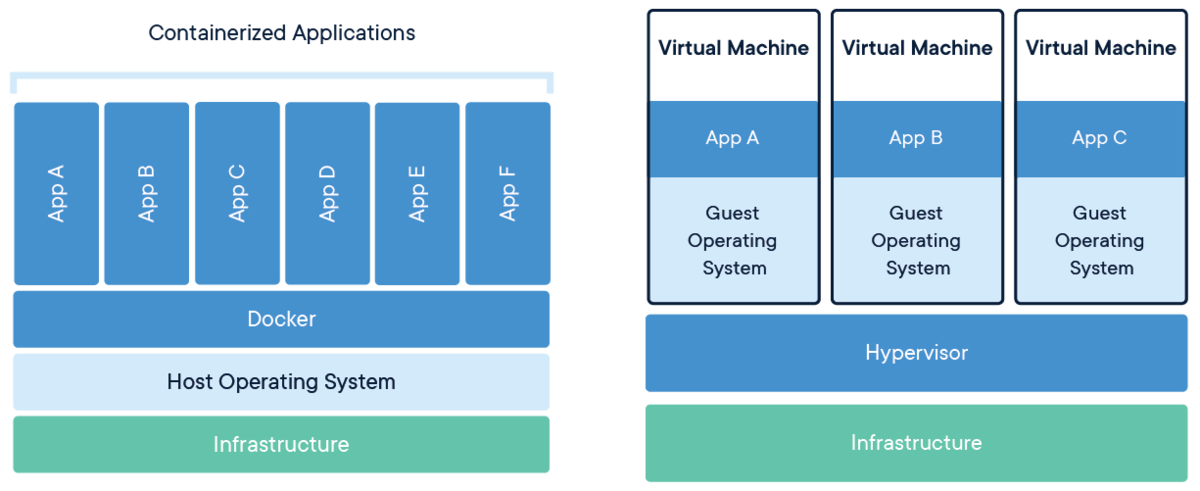
\includegraphics[scale=0.25]{immagini/docker-containerized-and-vm-transparent-bg.png}
    \caption{Stratificazione di un sistema a container e di un sistema con VMs}
    \label{fig:container-vs-VM}
\end{figure}
\chapter{Installazione}
\label{Installazione}
\thispagestyle{plain}

%\section{Introduzione}
L'installazione di ShareLaTeX è stata fatta su una macchina virtuale ospitata da un server del laboratorio AImageLab. Tale macchina ha nome \verb|sharelatex| ed esegue il sistema operativo Ubuntu 18.04 LTS, il più recente alla data corrente. Il sistema è accessibile sia dall'interno dell'ateneo (se collegati alla rete locale), sia dall'esterno, grazie all'apertura della porta 443, all'indirizzo \url{sharelatex.ing.unimore.it}. L'installazione e la configurazione sono avvenute seguendo i passi sotto riportati. L'attuale amministratore del sistema è il Dott. Federico Bolelli.

\section{Docker}
Per il progetto ShareLaTeX si è optato per l'installazione di Docker CE, in quanto non risultano necessarie le funzionalità aggiuntive dell'Enterprise Edition, rivolte invece alle grandi imprese. L'installazione può avvenire in diversi modi, come indicato nella guida ufficiale \cite{docker_install}. Si è scelto di utilizzare il metodo raccomandato da Docker, ovvero tramite i loro repository.

\subsection{Download}
Aggiornare l'indice dei pacchetti di \verb|apt-get|:
\begin{lstlisting}
sudo apt-get update
\end{lstlisting}
Installare i pacchetti necessari per permettere a \verb|apt-get| di utilizzare un repository su HTTPS:
\begin{lstlisting}
sudo apt-get install \ 
    apt-transport-https \
    ca-certificates \
    curl \
    software-properties-common
\end{lstlisting}
Aggiungere la chiave GPG ufficiale di Docker:
\begin{lstlisting}
curl -fsSL https://download.docker.com/linux/ubuntu/gpg | sudo apt-key add -
\end{lstlisting}
Verificare di possedere la chiave con la fingerprint\\
\verb|9DC8 5822 9FC7 DD38 854A E2D8 8D81 803C 0EBF CD88|\\
confrontando gli ultimi 4 byte della fingerprint:
\begin{lstlisting}
sudo apt-key fingerprint 0EBFCD88
\end{lstlisting}
che dovrebbe produrre un output simile al seguente:
\begin{lstlisting}
pub   4096R/0EBFCD88 2017-02-22
Key fingerprint = 9DC8 5822 9FC7 DD38 854A E2D8 8D81 803C 0EBF CD88
uid     Docker Release (CE deb) <docker@docker.com>
sub     4096R/F273FCD8 2017-02-22
\end{lstlisting}
Montare il repository specificando l'architettura (in questo caso x64):
\begin{lstlisting}
sudo add-apt-repository \
"deb [arch=amd64] https://download.docker.com/linux/ubuntu \
$(lsb_release -cs) \
stable"
\end{lstlisting}

\subsection{Installazione}
Installare l'ultima versione di Docker CE:
\begin{lstlisting}
sudo apt-get install -y docker-ce
\end{lstlisting}
Verificare che Docker CE sia installato correttamente avviando l'immagine \verb|hello-world|:
\begin{lstlisting}
sudo docker run hello-world
\end{lstlisting}


\section{Docker Compose}
Docker Compose non è incluso all'interno di Docker CE. La sua installazione è necessaria ai fini del progetto per poter gestire i tre container che strutturano l'applicazione: ShareLaTeX, MongoDB e Redis.
\begin{figure}[h]
    \centering
    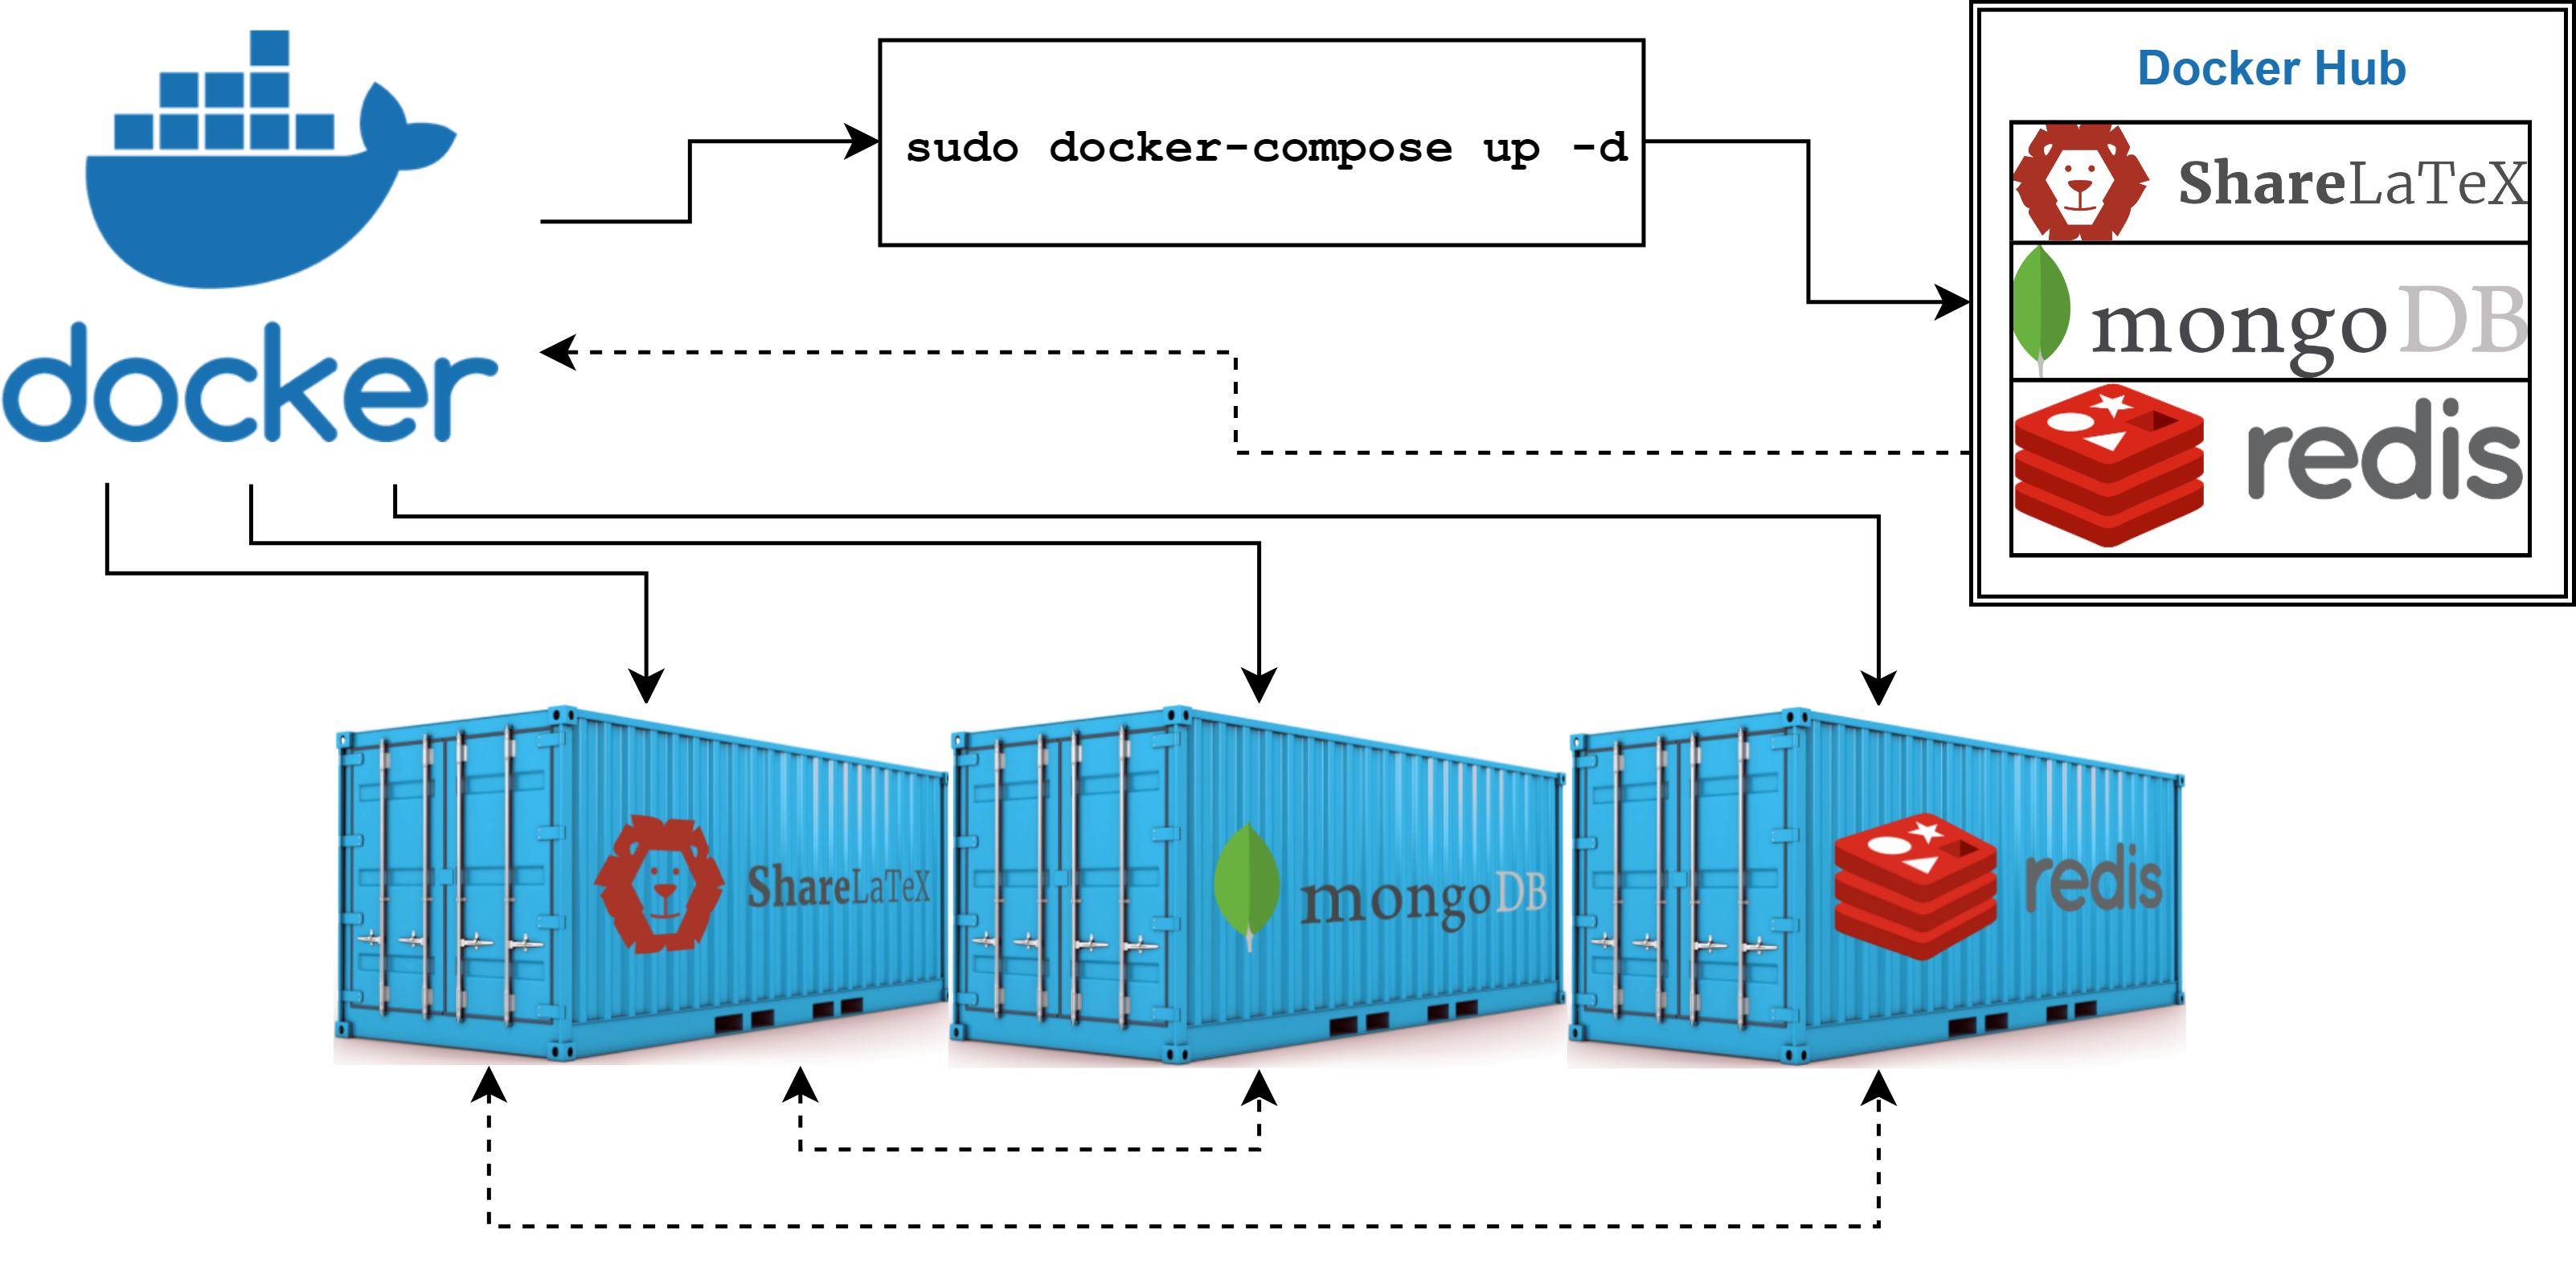
\includegraphics[width=\textwidth]{immagini/docker_container_dependencies.png}
    \caption{Esecuzione di Docker Compose e dipendenze fra container}
    \label{fig:docker_compose_dipendenze}
\end{figure}

\subsection{Download e installazione}
Con il comando che segue è possibile scaricare la versione 1.21.2 di Docker Compose. Per installare un'altra versione del software, eventualmente più aggiornata, è necessario modificare l'URL inserendo la versione richiesta \cite{docker_compose_release}.
\begin{lstlisting}
sudo curl -L https://github.com/docker/compose/releases/download/1.21.2/docker-compose-$(uname -s)-$(uname -m) -o /usr/local/bin/docker-compose
\end{lstlisting}
Occorre quindi applicare i permessi di esecuzione al file binario:
\begin{lstlisting}
sudo chmod +x /usr/local/bin/docker-compose
\end{lstlisting}
e testare l'installazione:
\begin{lstlisting}
docker-compose --version
\end{lstlisting}

\subsection{Configurazione}
Creare una directory dal nome \verb|sharelatex| e inserirvi \verb|docker-compose.yml|. Il template fornito dagli sviluppatori di ShareLaTeX per l'installazione tramite Docker è il seguente:
\lstinputlisting[caption={Template di docker-compose.yml}, captionpos=b, label=code:docker-compose.yml]{script/docker-compose-ridotto.yml}
Oltre a creare il container di ShareLaTeX, il file configura MongoDB e Redis. Inoltre fornisce una buona interfaccia per fornire impostazioni a ShareLaTeX\footnote{Approfondimento nel capitolo \hyperref[Configurazione]{\enquote*{Configurazione}}.}.
\begin{lstlisting}
mkdir sharelatex
cd sharelatex
wget https://raw.githubusercontent.com/aimagelab/sharelatex/master/docker-compose.yml
\end{lstlisting}
Infine avviare i container di ShareLaTeX, MongoDB e Redis usando le impostazioni di \verb|docker-compose.yml|. L'opzione \verb|-d| serve per avviare i container in modalità \enquote*{detached}, ovvero in background.
\begin{lstlisting}
sudo docker-compose up -d
\end{lstlisting}
Per visualizzare i container attualmente attivi, eseguire il comando:
\begin{lstlisting}
sudo docker ps
\end{lstlisting}

\section{TeX Live}
TeX Live \cite{texlive} è un distribuzione del sistema \TeX ~per installare, gestire e aggiornare pacchetti utilizzati per scrivere in \LaTeX. L'installazione completa dei pacchetti di TeX Live è essenziale per poter utilizzare qualsiasi pacchetto all'interno dei propri documenti. La totalità dei pacchetti occupa molta memoria sul disco (circa 7 GB), pertanto l'immagine di ShareLaTeX in Docker Hub presenta solo un'installazione parziale di TeX Live. La procedura di installazione richiederà molto tempo (circa 2 ore). L'immagine utilizzata per il container ShareLaTeX contiene la versione 2017 di TeX Live. Per l'installazione completa dei pacchetti di TeX Live 2018 e la risoluzione dei conflitti dei pacchetti preinstallati versione 2017, si è seguita la guida di aggiornamento fornita da TeX Live \cite{texlive_upgrade}.

\subsection{Fasi preliminari}
Modificare la variabile d'ambiente \verb|PATH|. Il modo più efficace e persistente consiste nell'aggiunta di \verb|PATH| fra le variabili d'ambiente di ShareLaTeX in \verb|docker-compose.yml|:
\begin{lstlisting}
environment:
    PATH: /usr/local/sbin:/usr/local/bin:/usr/sbin:/usr/bin:/sbin:/bin:/usr/local/texlive/2018/bin/x86_64-linux
\end{lstlisting}
Si ricorda che il ripristino/ricreazione di un qualunque container eliminerà tutte le modifiche ad esso apportate. Ciò significa che un eventuale riavvio del container ShareLaTeX dopo l'installazione completa di TeX Live ripristinerebbe lo stato dell'installazione iniziale. Questo può succedere, ad esempio, a seguito di modifiche al file \verb|docker-compose.yml| e all'esecuzione di \verb|sudo docker-compose up -d|. Pertanto è opportuno montare un volume esterno in corrispondenza della directory \verb|/usr/local/texlive/2018| per rendere persistenti i file dell'aggiornamento:
\begin{lstlisting}
volumes:
    - ~/sharelatex_texlive:/usr/local/texlive/2018
\end{lstlisting}
Salvare quindi le modifiche e riavviare i container:
\begin{lstlisting}
sudo docker-compose up -d
\end{lstlisting}

\subsection{Aggiornamento}
Per eseguire l'aggiornamento è necessario avviare una bash all'interno del container ShareLaTeX. Docker permette di avviare comandi all'interno dei container mediante il comando \verb|exec|. Le opzioni \verb|-t| e \verb|-i| servono rispettivamente per creare una pseudo-TTY e per renderla interattiva:
\begin{lstlisting}
sudo docker exec -ti sharelatex bash
\end{lstlisting}
Una volta all'interno del container, visitare il percorso \verb|/usr/local/texlive| e copiare il contenuto della directory \verb|2017| in \verb|2018|, generata dopo aver montato il volume e riavviato il container:
\begin{lstlisting}
cd /usr/local/texlive
cp -a 2017/* 2018
cd 2018
\end{lstlisting}
Scaricare ed eseguire lo script d'aggiornamento \verb|update-tlmgr-latest.sh|:
\begin{lstlisting}
wget http://ctan.mirror.garr.it/mirrors/CTAN/systems/texlive/tlnet/update-tlmgr-latest.sh
sh update-tlmgr-latest.sh -- --upgrade
tlmgr update --self --all
\end{lstlisting}
Ripristinare la cache lualatex/fontspec:
\begin{lstlisting}
luaotfload-tool -fu
\end{lstlisting}
Infine uscire dal container con \verb|exit|.

\subsection{Installazione}
L'installazione completa di TeX Live sarà avviata tramite il comando \verb|exec| dall'esterno (l'operazione richiederà molto tempo):
\begin{lstlisting}
sudo docker exec sharelatex tlmgr install scheme-full
\end{lstlisting}
Attendere fino al termine dell'installazione. Eventuali interruzioni non comprometteranno l'installazione, che potrà ricominciare da dove era stata interrotta rilanciando il comando precedente.

\section{NGINX reverse proxy}
NGINX \cite{nginx} è un software open source che può essere utilizzato come web server, strumento di caching, load balancer, media streamer, ma anche come reverse proxy. In questo paragrafo si vedrà come installare e configurare un reverse proxy NGINX per utilizzare il protocollo HTTPS con ShareLaTeX. Per far ciò è stato necessario ottenere certificato e chiave SSL (Secure Sockets Layer), entrambi forniti dall'amministratore di rete del dipartimento e disponibili sulla macchina nella directory \verb|sharelatex.ing.unimore.it|.

\subsection{Installazione}
NGINX sarà installato tramite Docker. Si utilizzerà l'immagine \verb|jwilder/nginx-proxy| \cite{nginx-proxy}, che configura un container con NGINX e \emph{docker-gen}. Questo è un generatore di file che creaconfigurazioni per NGINX, per adattare il reverse proxy a seconda dei container attivi. Quindi bisogna includere in \verb|docker-compose.yml| il nuovo container:
\begin{lstlisting}
nginx-proxy:
        image: jwilder/nginx-proxy
        container_name: nginx-proxy
        ports:
            - "443:443"
        volumes:
            - /var/run/docker.sock:/tmp/docker.sock:ro
            - /home/sharelatex/tmp:/etc/nginx/certs
\end{lstlisting}
È necessario montare i volumi esterni necessari per rendere persistente la configurazione del proxy server. Le directory interessate sono \verb|sharelatex.ing.unimore.it| e \verb|nginx_confd|:
\begin{lstlisting}
            - ~/sharelatex.ing.unimore.it:/etc/nginx/cert
            - ~/nginx_confd:/etc/nginx/conf.d
\end{lstlisting}
Successivamente, aggiungere tre variabili d'ambiente a ShareLaTeX:
\begin{itemize}
    \item \verb|VIRTUAL_HOST|: indica l'indirizzo IP con cui il proxy può raggiungere il container ShareLaTeX.
    \item \verb|SHARELATEX_SECURE_COOKIE|: abilita lo scambio di Secure Cookie fra client e server.
    \item \verb|SHARELATEX_BEHIND_PROXY|: notifica all'applicazione dell'esistenza del proxy.
\end{itemize}
\begin{lstlisting}
VIRTUAL_HOST: 103.112.212.22
SHARELATEX_SECURE_COOKIE: 'true'
SHARELATEX_BEHIND_PROXY: 'true'
\end{lstlisting}
Riavviare successivamente i container:
\begin{lstlisting}
sudo docker-compose up -d
\end{lstlisting}

\subsection{Configurazione}
Esplorare la directory \verb|nginx_confd|. Sarà presente il file \verb|default.conf|, generato dal container. Questo file configura il proxy includendo qualsiasi file con estensione \verb|.conf|. Scaricare quindi il file \verb|sharelatex.conf|:
\begin{lstlisting}
cd nginx_confd
wget https://raw.githubusercontent.com/aimagelab/sharelatex/master/sharelatex.conf
\end{lstlisting}
Il file è il seguente:
\lstinputlisting[caption={sharelatex.conf}, captionpos=b, style=my-style]{script/sharelatex.conf}
Si configura il server per ascoltare sulla porta 443, abilitando SSL, indicando certificato e chiave SSL. È importante indicare \verb|proxy_pass http://103.112.212.22|, per inoltrare tutto il traffico all'indirizzo IP 103.112.212.22, che corrisponde al \verb|VIRTUAL_HOST| di ShareLaTeX.
\chapter{Configurazione}
\label{Configurazione}
\thispagestyle{plain}

\section{Primo avvio}
Una volta eseguito Docker Compose, il sistema risulta avviato, funzionante e raggiungibile sulla porta 80, dall'host all'indirizzo \verb|localhost|, oppure da una macchina collegata alla rete locale tramite \verb|hostname|. Per quanto riguarda l'installazione fatta in ateneo, la macchine è raggiungibile all'indirizzo \verb|sharelatex.ing.unimore.it|, che verrà preso come esempio per i passi successivi.

\subsection{Registrazione dell'amministratore}
\begin{figure}[h]
    \begin{subfigure}{0.5\textwidth}
        \centering
        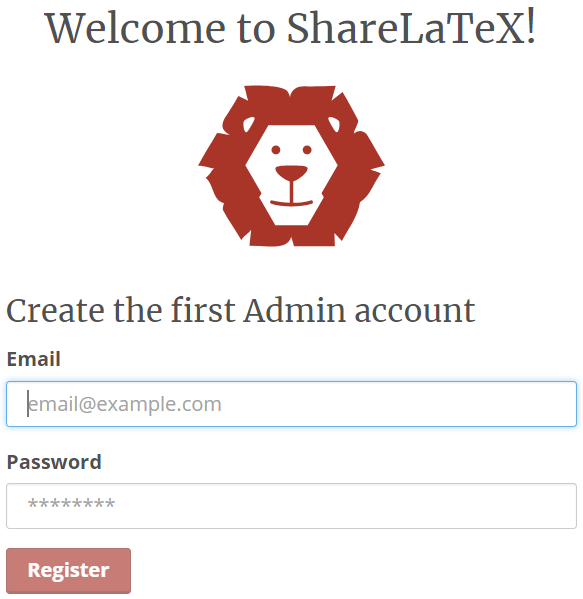
\includegraphics[height=6cm]{immagini/launchpad_1.png}
        \caption{Launchpad}
        \label{fig:sharelatex_launchpad_1}
    \end{subfigure}
    \begin{subfigure}{0.5\textwidth}
        \centering
        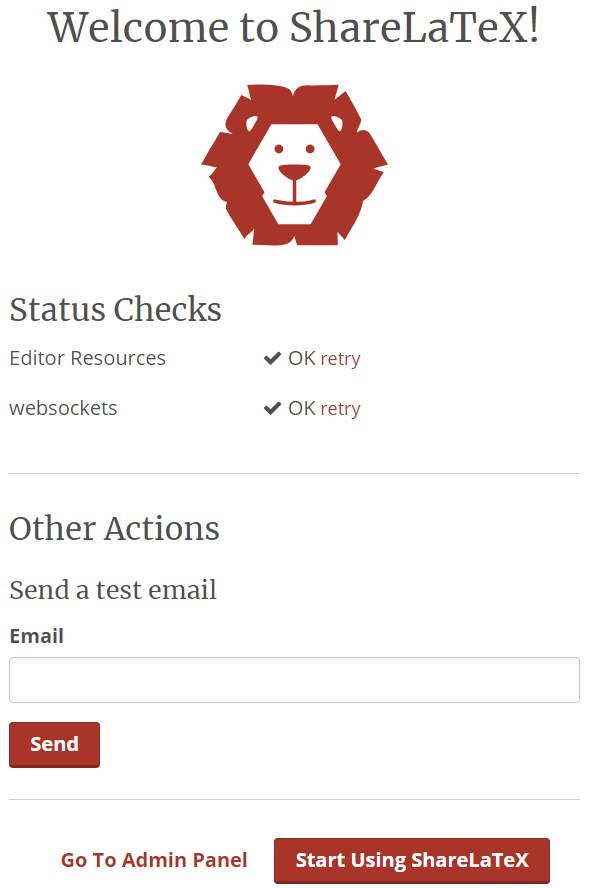
\includegraphics[height=6cm]{immagini/launchpad_2.png}
        \caption{Schermata di controllo}
        \label{fig:sharelatex_launchpad_2}
    \end{subfigure}
    \caption{Creazione utente amministratore}
    \label{fig:sharelatex_launchpad}
\end{figure}
\noindent Per registrare l'amministratore del sistema, visitare la pagina all'indirizzo\\\verb|sharelatex.ing.unimore.it/launchpad|. Una volta inseriti indirizzo e-mail e password dell'amministratore, verrà richiesto il primo login. Inserite le credenziali dell'amministratore, verrà mostrato il launchpad, il quale mostra lo stato dell'editor e delle websocket e dal quale è possibile inviare un'email di test a un indirizzo a scelta\footnote{Per usufruire di questa funzionalità è necessario configurare il servizio mail con \hyperref[SMTP]{SMTP}.}.

\subsection{Gestione utenti}
L'amministratore può registrare utenti normali all'applicazione aggiungendo la loro email nella pagina \enquote*{Manage Users}. La piattaforma genera un link per impostare la password del nuovo account.

Per eliminare un utente e tutti i progetti salvati sul suo account è invece necessario eseguire il seguente comando, indicando l'indirizzo mail dell'account da eliminare:
\begin{lstlisting}
sudo docker exec sharelatex /bin/bash -c "cd /var/www/sharelatex; grunt user:delete --email user@sharelatex.com"
\end{lstlisting}

\section{Interfaccia}
\verb|docker-compose.yml| permette anche di impostare variabili d'ambiente all'interno dei container. ShareLaTeX è altamente configurabile sotto questo aspetto. Si elencano le variabili d'ambiente utilizzate per l'installazione in ateneo:
\begin{itemize}
    \item \verb|SHARELATEX_APP_NAME|: nome dell'applicazione, che sarà mostrato nella barra di navigazione del browser.
    \item \verb|SHARELATEX_NAV_TITLE|: nome dell'applicazione, che sarà mostrato in alto a sinistra nell'homepage del profilo utente.
    \item \verb|SHARELATEX_HEADER_IMAGE|: URL di un'immagine, che sarà mostrata in alto a sinistra. Nel caso in cui \verb|SHARELATEX_NAV_TITLE| fosse impostato, allora\\\verb|SHARELATEX_HEADER_IMAGE| avrà la priorità.
    \item \verb|SHARELATEX_SITE_URL|: indirizzo della macchina host del servizio.
    \item \verb|SHARELATEX_ADMIN_EMAIL|: indirizzo e-mail dell'amministratore di sistema, che sarà mostrata in fase di registrazione utente.
    \item \verb|SHARELATEX_LEFT_FOOTER|: array JSON in cui si può aggiungere testo HTML che verrà mostrato in basso a sinistra nell'homepage.
    \item \verb|SHARELATEX_RIGHT_FOOTER|: array JSON in cui si può aggiungere testo HTML che verrà mostrato in basso a destra nell'homepage.
    \item \verb|SHARELATEX_SITE_LANGUAGE|: lingua dell'applicazione. Di default la lingua impostata è inglese, ma sono disponibili anche:
        \begin{multicols}{3}
            \begin{itemize}
                \item es = spagnolo
                \item pt = portoghese
                \item de = tedesco
                \item fr = francese
                \item cs = ceco
                \item nl = olandese
                \item sv = svedese
                \item it = italiano
                \item tr = turco
                \item cn = cinese
                \item no = norvegese
                \item da = danese
                \item ru = russo
                \item ko = coreano
                \item ja = giapponese
            \end{itemize}
        \end{multicols}
\end{itemize}

\section{SMTP}
\label{SMTP}
In fase di registrazione di un nuovo utente, come si è già detto, viene generato un link di iscrizione. Tale link deve essere in qualche modo consegnato al nuovo utente. Se il servizio email è configurato, allora questa fase sarà automatica. I parametri sono passati mediante variabili d'ambiente. Si raccomanda di impostare \verb|SHARELATEX_SITE_URL| per generare link di iscrizione funzionanti. Si elencano le variabili d'ambiente utilizzate per l'installazione in ateneo:
\begin{itemize}
    \item \verb|SHARELATEX_EMAIL_FROM_ADDRESS|: indirizzo del mittente del messaggio.
    \item \verb|SHARELATEX_EMAIL_SMTP_HOST|: host del servizio SMTP.
    \item \verb|SHARELATEX_EMAIL_SMTP_PORT|: porta SMTP da utilizzare.
    \item \verb|SHARELATEX_EMAIL_SMTP_SECURE|: valore booleano che, se vero, attiva SMTPS.
    \item \verb|SHARELATEX_EMAIL_SMTP_USER|: nome utente da autenticare.
    \item \verb|SHARELATEX_EMAIL_STMP_PASS|: password dell'utente da autenticare.
    \item \verb|SHARELATEX_EMAIL_STMP_TLS_REJECT_UNAUTH|: valore booleano che, se vero, rifiuta connessioni TLS (Transport Layer Security) non autorizzate.
    \item \verb|SHARELATEX_EMAIL_STMP_IGNORE_TLS|: valore booleano che, se vero, disattiva il supporto STARTTLS.
    \item \verb|SHARELATEX_CUSTOM_EMAIL_FOOTER|: testo HTML con cui si può personalizzare il footer delle email.
\end{itemize}
\chapter{Manutenzione}
\label{Manutenzione}
\thispagestyle{empty}

In questa capitolo si spiega come provvedere a conservare lo stato dell'installazione locale di ShareLaTeX. È necessario pianificare le attività di ripristino dei dati del sistema in quanto l'avvio dei container con immagini aggiornate potrebbe impedire il corretto funzionamento del sistema o la perdita di dati e documenti finora creati. Si ricorda inoltre che un semplice riavvio dei container comporta il loro ripristino.

\section{Backup e ripristino}
Il \href{code:docker-compose.yml}{template} di \verb|docker-compose.yml| mostrato nel capitolo Installazione possiede già impostazioni riguardanti la persistenza dei dati dei tre container installati. Saranno aggiunte altre impostazioni per rendere più sicura la procedura di aggiornamento del sistema in futuro.

\subsection{MongoDB}
MongoDB possiede due tool chiamati \verb|mongodump| e \verb|mongorestore| che saranno utilizzati per esportare ed importare il dataset in un formato sicuro per il backup. Per ulteriori informazioni visitare la documentazione ufficiale di MongoDB all'indirizzo \url{https://docs.mongodb.com/manual/tutorial/backup-and-restore-tools/}. Innanzitutto eseguire \verb|mongodump|.
\begin{lstlisting}
sudo docker exec mongo mongodump
\end{lstlisting}
L'output sarà all'interno del container MongoDB in \verb|/dump|. Per rendere questi file persistenti occorre montare un volume esterno. Si noti che Il template di \verb|docker-compose.yml| crea di default un volume per la persistenza dei dati, che non è sufficiente in caso di upgrade o downgrade di MongoDB.
\begin{lstlisting}
volumes:
    - ~/mongo_data:/data/db
    - ~/mongodump_data:/dump
\end{lstlisting}
Riavviando il container l'output di \verb|mongodump| sarà accessibile nella home directory dell'host. Con \verb|mongorestore| sarà poi possibile ripristinare lo stato di MongoDB.
\begin{lstlisting}
sudo docker exec mongo mongorestore /dump
\end{lstlisting}

\subsection{Redis}
Redis contiene dati a breve termine, ma può essere comunque importante eseguire un backup dei dati. Il template di \verb|docker-compose.yml| crea di default un volume per la persistenza dei dati. Conterrà un unico file nominato \verb|dump.rdb|.
\begin{lstlisting}
volumes:
    - ~/redis_data:/data
\end{lstlisting}

\subsection{ShareLaTeX}
I dati relativi a ShareLaTeX sono salvati all'interno del container in \verb|/var/lib/sharelatex| e il template di \verb|docker-compose.yml| crea di default un volume per la persistenza dei dati.
\begin{lstlisting}
volumes:
    - ~/sharelatex_data:/var/lib/sharelatex
\end{lstlisting}

\section{Aggiornamento}
Una volta eseguiti i passi per gestire l'operazione di backup e ripristino è necessario definire gli step per eseguire l'upgrade (o downgrade) dei container in modo sicuro, senza perdita di dati.

\subsection{Lougout degli utenti}
È opportuno impedire agli utenti di utilizzare l'applicazione durante la fase di aggiornamento. Per far ciò l'amministratore deve fare login e accedere al pannello di gestione del sito presso \verb|sharelatex.ing.unimore.it/admin|.
\begin{figure}[h]
    \centering
    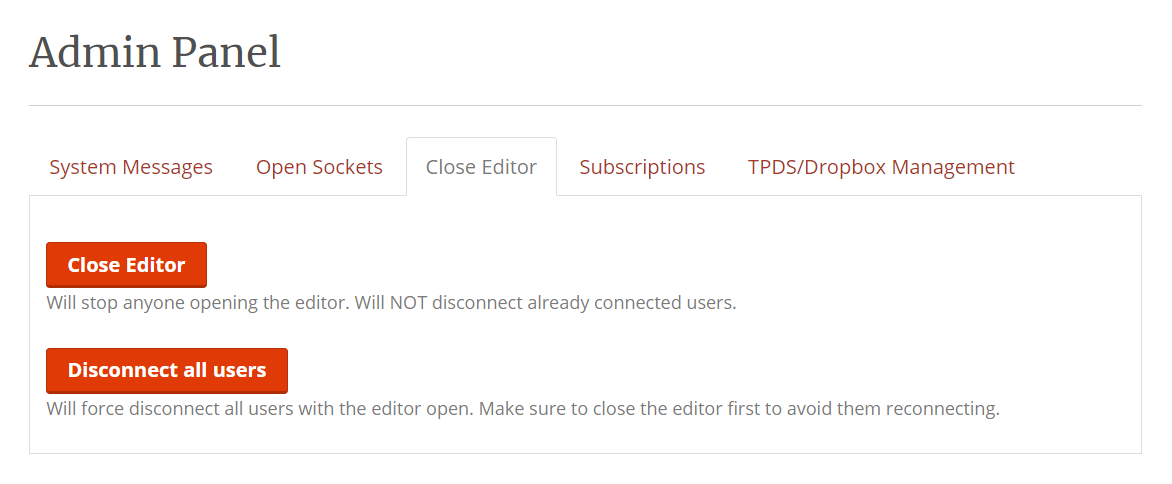
\includegraphics[width=\textwidth]{immagini/close_editor.PNG}
    \caption{Pannello di controllo dell'amministratore}
    \label{fig:close_editor}
\end{figure}
\begin{enumerate}
    \item Accedere alla scheda \enquote*{Close Editor}.
    \item Cliccare sul bottone \enquote*{Close Editor}: impedisce agli utenti di caricare l'editor di progetto.
    \item Cliccare sul bottone \enquote*{Disconnect all users}: chiunque sia connessio all'editor verrà rinviato ad una pagina di avviso manutenzione.
\end{enumerate}
L'unico modo per riavviare l'editor consiste nel riavvio dei container.

\subsection{Esecuzione di mongodump}
Per eseguire il backup dei dati di MongoDB bisogna eseguire \verb|mongodump|. Non sarà necessario conservare la directory \verb|mongo_data| in quanto \verb|mongorestore| sarà in grado di ripristinarla a dovere. L'output di \verb|mongodump| avverrà in \verb|/dump| all'interno del container. Avendo montato un volume in \verb|~/mongodump_data|, tale percorso sarà accessibile dall'esterno del container e persistente.
\begin{lstlisting}
sudo docker exec mongo mongodump
\end{lstlisting}

\subsection{Sospensione e rimozione dei container}
Si può scegliere se agire su tutti e tre i container o solo sul container da aggiornare.
\begin{lstlisting}
sudo docker stop sharelatex mongo redis
sudo docker rm sharelatex mongo redis
\end{lstlisting}

\subsection{Rimozione dei dati precedenti}
Eliminare la directory sull'host \verb|mongo_data|. È necessario in quanto i container possono rifiutare l'avvio con dati diversi: è il caso di MongoDB. Non bisogna eliminare invece la directory sull'host \verb|mongodump_data| perché frutto del montaggio di un volume esterno necessario per eseguire \verb|mongorestore|.
\begin{lstlisting}
sudo rm -r ~/mongo_data
\end{lstlisting}
Se al successivo riavvio del sistema il container Redis dovesse rifiutare il riavvio, aggiungere agli step precedenti l'eliminazione della diretory sull'host \verb|redis_data|.
\begin{lstlisting}
sudo rm -r ~/redis_data
\end{lstlisting}

\subsection{Riavvio del sistema}
Il template di \verb|docker-compose.yml| imposta come immagine di default per ogni container quella con tag \verb|latest|. È possibile anche selezionare una specifica immagine da scaricare. L'elenco delle immagini disponibili è su Docker Hub. Ad esempio, se si vuole l'immagine \verb|v1.0.0| di ShareLaTeX è necessario appendere il tag selezionato nel campo \verb|image| mediante \verb|:|. Segue un esempio di quanto detto.
\begin{lstlisting}
services:
    sharelatex:
        restart: always
        image: sharelatex/sharelatex:v1.0.0
        container_name: sharelatex
\end{lstlisting}
Quindi riavviare i container.
\begin{lstlisting}
sudo docker-compose up -d
\end{lstlisting}

\subsection{Ripristino con mongorestore}
Ci si presenterà una nuova installazione dell'applicazione. Per ripristinare i dati precedenti occorre eseguire \verb|mongorestore|.
\begin{lstlisting}
sudo docker exec mongo mongorestore /dump
\end{lstlisting}

\section{Automatizzazione degli aggiornamenti: update.sh}
Per automatizzare il processo di aggiornamento dei container è stato prodotto lo script \verb|update.sh|. Questo script esegue il procedimento precedentemente descritto passo per passo, mostrando all'utente lo stato di ogni fase. Per eseguire lo script è necessario scaricarlo e ottenere i permessi di esecuzione.
\begin{lstlisting}
wget https://raw.githubusercontent.com/aimagelab/sharelatex/master/update.sh
chmod +x update.sh
\end{lstlisting}
Lo script accetta un parametro che identifica una directory. Tale directory deve contenere un file \verb|docker-compose.yml| da utilizzare per avviare e configurare i container.
\begin{lstlisting}
# Utilizzo
./update.sh <dir>
\end{lstlisting}
Lo script controlla innanzitutto il numero dei parametri: se non sufficiente, allora lo notifica all'utente. Esegue quindi un controllo sul parametro, per verificare che identifichi una directory traversabile. Segue eseguendo \verb|mongodump|, arrestando i container, eliminando i dati superflui, riavviando i container, per poi ripristinare i dati con \verb|mongorestore|. Mostra infine lo stato attuale dei container attivi e chiede all'utente se proseguire con l'installazione completa (o aggiornamento) di TeX Live.

Si raccomanda di utilizzare questo script anche in caso di semplice riavvio dei container: dato che è stato impostato in \verb|docker-compose.yml| che l'immagine da utilizzare per la creazione dei container è quella con tag \enquote*{latest}, l'eventuale release di un'immagine aggiornata comporterebbe il suo download la sostituzione con l'immagine precedente, il che costituisce un vero e proprio aggiornamento.

Segue lo script \verb|update.sh|
\lstinputlisting[caption={Script update.sh}, captionpos=b, style=my-style]{script/update-ridotto.sh}





\cleardoublepage
% ---- Bibliography ----
%\addcontentsline{toc}{chapter}{Bibliografia}
%\bibliographystyle{plain}
%\bibliography{bibl_tesi}
%\nocite{*}

\end{document}





